\subsubsection*{Level 1}



In this section, we need to design the linear friction $d_1$ in the friction model $M_f = d_1 \dot{\varphi}$ and the total inertia $J$.

The parameter identification is done using a step time $T_s = 1 \text{ ms}$.

In order to do so, we add our motor model to the ControlDesk. We then fit the theoretical curve to the real one (using sliders to modify $d_1$ and $J$). 

The fitted curves for motor 1 and motor 2 are on Figure \ref{fittedCurves}. %The real curves are oscillating, due to ????

We have the following values:

\begin{center}
\begin{tabular}{|c|c|c|}
 \hline
 & Motor 1 & Motor 2 \\
 \hline 
 $J$ & $4.16e-7$ & $4.16e-7$ \\ 
 \hline 
 $d_1$ & $4.2e-6$ & $4.4e-6$  \\
 \hline
\end{tabular}
\end{center}


\begin{center}
\begin{figure}[Ht]
 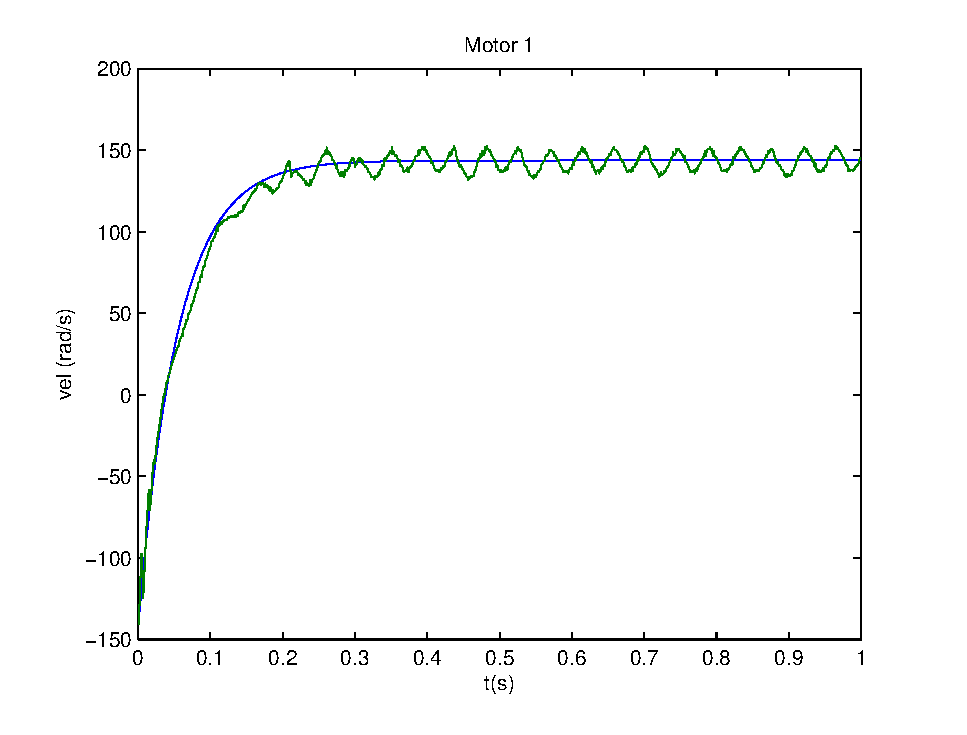
\includegraphics[width=\linewidth]{fig/motor1L1.eps}
 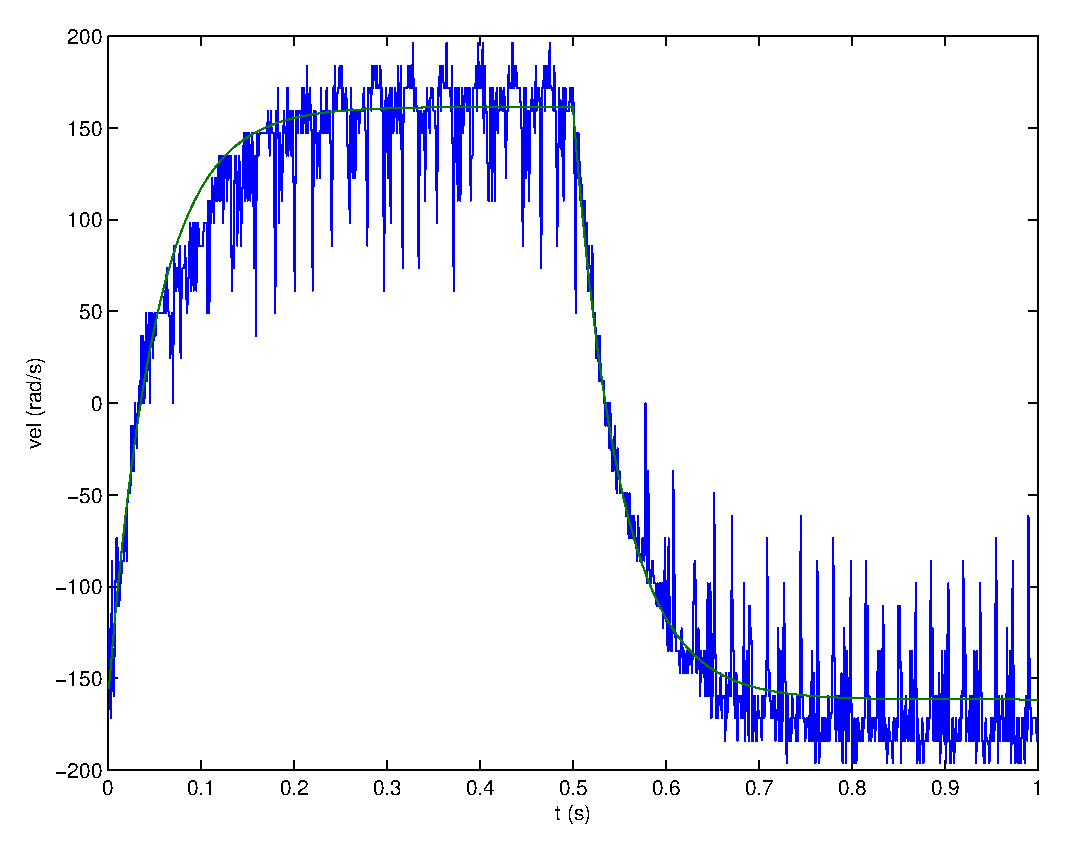
\includegraphics[width=\linewidth]{fig/motor2L1.eps}
 \caption{Fitted curves for motor 1 \& 2 -- blue\\ Real curves for motor 1 \& 2 -- green}
 \label{fittedCurves}
\end{figure}
\end{center}



\subsubsection*{Level 2}

blabla...